\documentclass[tikz,border=12pt]{standalone}
\usepackage{tikz}
\begin{document}
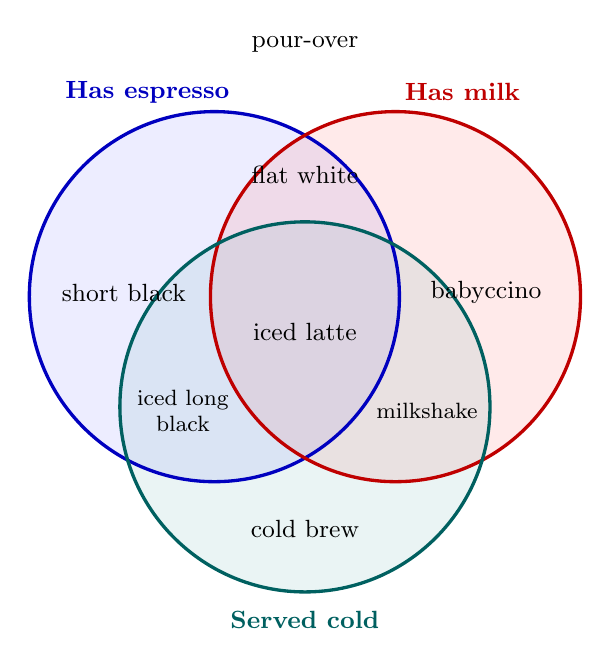
\begin{tikzpicture}[font=\sffamily]
  % The three sets
  \fill[blue!55,fill opacity=0.13] (-1.15,0.1) circle (2.35);
  \fill[red!65,fill opacity=0.13] (1.15,0.1) circle (2.35);
  \fill[teal!65,fill opacity=0.13] (0,-1.3) circle (2.35);
  \draw[blue!75!black,line width=1.2pt] (-1.15,0.1) circle (2.35);
  \draw[red!75!black,line width=1.2pt] (1.15,0.1) circle (2.35);
  \draw[teal!75!black,line width=1.2pt] (0,-1.3) circle (2.35);

  % Drinks, positioned in their respective intersections
  \node[align=center,font=\small] at (-2.3,0.15) {short black};
  \node[align=center,font=\small] at (2.3,0.15) {babyccino};
  \node[align=center,font=\small] at (0,1.65) {flat white};
  \node[align=center,font=\small] at (0,-0.35) {iced latte};
  \node[align=center,font=\footnotesize] at (-1.55,-1.35) {iced long\\black};
  \node[align=center,font=\footnotesize] at (1.55,-1.35) {milkshake};
  \node[align=center,font=\small] at (0,-2.85) {cold brew};
  \node[align=center,font=\small] at (0,3.3) {pour-over};

  % Set labels outside the circles
  \node[blue!75!black,font=\small\bfseries] at (-2.0,2.7) {Has espresso};
  \node[red!75!black,font=\small\bfseries] at (2.0,2.7) {Has milk};
  \node[teal!75!black,font=\small\bfseries,align=center] at (0,-4.0) {Served cold};
\end{tikzpicture}
\end{document}
